% 第十一章：分离变量法\index{分离变量法}

\chapter{分离变量法\index{分离变量法}}

\begin{wulibj}[本章导读]
分离变量法\index{分离变量法}是求解数学物理方程最重要、最常用的方法之一。其基本思想是将多变量问题分解为若干单变量问题。本章我们将以一维波动方程为例，详细讲解分离变量法\index{分离变量法}的基本步骤，并推广到热传导方程和拉普拉斯方程。
\end{wulibj}

% ========== 第一节 ==========
\section{分离变量法\index{分离变量法}的基本思想}

\subsection{问题的提出}

考虑有界弦的自由振动问题：
\begin{equation}
    \begin{cases}
        \dfrac{\partial^2 u}{\partial t^2} = a^2\dfrac{\partial^2 u}{\partial x^2}, & 0 < x < l, \; t > 0 \\
        u(0, t) = u(l, t) = 0, & t \geq 0 \\
        u(x, 0) = \varphi(x), \quad \dfrac{\partial u}{\partial t}(x, 0) = \psi(x), & 0 \leq x \leq l
    \end{cases}
\end{equation}

\subsection{分离变量的基本步骤}

\textbf{第一步：设分离变量形式的解}

设解可以写成单变量函数的乘积：
\begin{equation}
    u(x, t) = X(x)T(t)
\end{equation}

\textbf{第二步：代入方程，分离变量}

代入波动方程：
\begin{equation}
    X(x)T''(t) = a^2 X''(x)T(t)
\end{equation}

分离变量：
\begin{equation}
    \frac{T''(t)}{a^2 T(t)} = \frac{X''(x)}{X(x)} = -\lambda
\end{equation}

由于左边只依赖于 $t$，右边只依赖于 $x$，要使等式对所有的 $x, t$ 成立，它们必须等于同一个常数 $-\lambda$。

\textbf{第三步：求解本征值问题}

由边界条件 $u(0, t) = u(l, t) = 0$ 得 $X(0) = X(l) = 0$。

得到\textbf{Sturm-Liouville 问题}：
\begin{equation}
    \begin{cases}
        X''(x) + \lambda X(x) = 0 \\
        X(0) = X(l) = 0
    \end{cases}
\end{equation}

\textbf{第四步：求解时间方程}

\begin{equation}
    T''(t) + \lambda a^2 T(t) = 0
\end{equation}

\textbf{第五步：叠加所有特解，确定系数}

\begin{equation}
    u(x, t) = \sum_{n=1}^{\infty} X_n(x)T_n(t)
\end{equation}

利用初始条件确定系数。

\begin{figure}[htbp]
\centering
\begin{tikzpicture}[scale=0.8, 
    box/.style={rectangle, draw, rounded corners, minimum width=2.5cm, minimum height=0.8cm, align=center, fill=blue!10},
    arrow/.style={->, thick, >=stealth}]
    
    % 节点
    \node[box] (step1) at (0, 0) {设 $u = X(x)T(t)$};
    \node[box] (step2) at (0, -1.5) {代入方程};
    \node[box] (step3) at (-3, -3) {空间方程\\$X'' + \lambda X = 0$};
    \node[box] (step4) at (3, -3) {时间方程\\$T'' + \lambda a^2 T = 0$};
    \node[box, fill=orange!20] (step5) at (-3, -4.8) {本征值问题\\边界条件};
    \node[box, fill=green!20] (step6) at (3, -4.8) {求解 $T_n(t)$};
    \node[box, fill=red!20] (step7) at (0, -6.3) {叠加 $u = \sum X_n T_n$};
    \node[box] (step8) at (0, -7.8) {确定系数};
    
    % 箭头
    \draw[arrow] (step1) -- (step2);
    \draw[arrow] (step2) -- node[left] {$-\lambda$} (step3);
    \draw[arrow] (step2) -- node[right] {$-\lambda$} (step4);
    \draw[arrow] (step3) -- (step5);
    \draw[arrow] (step4) -- (step6);
    \draw[arrow] (step5) -- (step7);
    \draw[arrow] (step6) -- (step7);
    \draw[arrow] (step7) -- (step8);
    
    % 标注
    \node[gray] at (5, -3) {$\lambda_n$, $X_n$};
    \node[gray] at (5, -4.8) {$T_n(t)$};
\end{tikzpicture}
\caption{分离变量法求解流程}
\label{fig:separation-flowchart}
\end{figure}

% ========== 第二节 ==========
\section{本征值问题}

\subsection{本征值与本征函数}

\begin{dingliyi}{本征值问题}{}
形如
\begin{equation}
    \begin{cases}
        \mathcal{L}y = \lambda y \\
        \text{边界条件}
    \end{cases}
\end{equation}
的问题称为本征值问题。使问题有非零解的 $\lambda$ 称为\textbf{本征值}，对应的非零解称为\textbf{本征函数}。
\end{dingliyi}

\subsection{三类边界条件下的本征值问题}

\begin{dingli}{第一类边界条件的本征值问题}{}
本征值和本征函数为
\[
    \lambda_n = \left(\frac{n\pi}{l}\right)^2, \quad X_n(x) = \sin\frac{n\pi x}{l}, \quad n = 1, 2, 3, \ldots
\]
\end{dingli}

\begin{proof}
分三种情况讨论：

\textbf{情况一}：$\lambda < 0$，设 $\lambda = -\mu^2$（$\mu > 0$）

通解 $X(x) = C_1\mathrm{e}^{\mu x} + C_2\mathrm{e}^{-\mu x}$。

由 $X(0) = 0$ 得 $C_1 + C_2 = 0$。

由 $X(l) = 0$ 得 $C_1\mathrm{e}^{\mu l} + C_2\mathrm{e}^{-\mu l} = 0$。

联立解得 $C_1 = C_2 = 0$，只有零解。所以 $\lambda < 0$ 无本征值。

\textbf{情况二}：$\lambda = 0$

通解 $X(x) = C_1 + C_2x$。

由边界条件 $X(0) = X(l) = 0$ 得 $C_1 = C_2 = 0$，只有零解。

\textbf{情况三}：$\lambda > 0$，设 $\lambda = \mu^2$

通解 $X(x) = C_1\cos\mu x + C_2\sin\mu x$。

由 $X(0) = 0$ 得 $C_1 = 0$。

由 $X(l) = 0$ 得 $C_2\sin\mu l = 0$。

要得到非零解，需要 $C_2 \neq 0$，故 $\sin\mu l = 0$，即 $\mu l = n\pi$。

所以 $\mu_n = \frac{n\pi}{l}$，$\lambda_n = \left(\frac{n\pi}{l}\right)^2$，$X_n(x) = \sin\frac{n\pi x}{l}$。
\end{proof}

\begin{figure}[htbp]
\centering
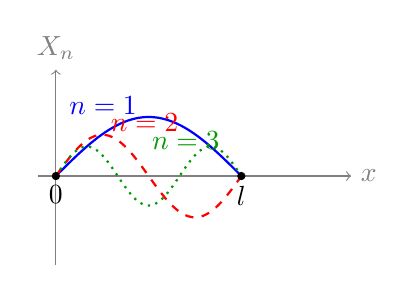
\begin{tikzpicture}[scale=0.75]
    % 坐标轴
    \draw[->, gray] (-0.3, 0) -- (5, 0) node[right] {$x$};
    \draw[->, gray] (0, -1.5) -- (0, 1.8) node[above] {$X_n$};
    
    % 刻度
    \node[below] at (0, 0) {$0$};
    \node[below] at (3.14, 0) {$l$};
    
    % n=1
    \draw[blue, thick, domain=0:3.14, samples=50] plot (\x, {sin(\x r)});
    \node[blue] at (0.8, 1.2) {$n=1$};
    
    % n=2
    \draw[red, thick, dashed, domain=0:3.14, samples=50] plot (\x, {0.7*sin(2*\x r)});
    \node[red] at (1.5, 0.9) {$n=2$};
    
    % n=3
    \draw[green!60!black, thick, dotted, domain=0:3.14, samples=50] plot (\x, {0.5*sin(3*\x r)});
    \node[green!60!black] at (2.2, 0.6) {$n=3$};
    
    % 节点标记
    \fill (0, 0) circle (2pt);
    \fill (3.14, 0) circle (2pt);
\end{tikzpicture}
\caption{第一类边界条件下的本征函数 $X_n(x) = \sin\frac{n\pi x}{l}$}
\label{fig:eigenfunctions-dirichlet}
\end{figure}

\begin{dingli}{第二类边界条件的本征值问题}{}
对于
\begin{equation}
    \begin{cases}
        X''(x) + \lambda X(x) = 0, \quad 0 < x < l \\
        X'(0) = X'(l) = 0
    \end{cases}
\end{equation}
本征值和本征函数为
\begin{equation}
    \boxed{\lambda_n = \left(\frac{n\pi}{l}\right)^2, \quad X_n(x) = \cos\frac{n\pi x}{l}, \quad n = 0, 1, 2, \ldots}
\end{equation}
注意：$n = 0$ 时，$\lambda_0 = 0$，$X_0(x) = 1$（常数解）。
\end{dingli}

\begin{proof}
类似地分三种情况讨论。

\textbf{情况一}：$\lambda < 0$，设 $\lambda = -\mu^2$

通解 $X(x) = C_1\mathrm{e}^{\mu x} + C_2\mathrm{e}^{-\mu x}$。由 $X'(0) = \mu(C_1 - C_2) = 0$ 得 $C_1 = C_2$。

由 $X'(l) = \mu(C_1\mathrm{e}^{\mu l} - C_2\mathrm{e}^{-\mu l}) = 0$ 得 $C_1(\mathrm{e}^{\mu l} - \mathrm{e}^{-\mu l}) = 0$。因 $\mu > 0$ 时 $\mathrm{e}^{\mu l} \neq \mathrm{e}^{-\mu l}$，故 $C_1 = 0$，只有零解。

\textbf{情况二}：$\lambda = 0$

通解 $X(x) = C_1 + C_2x$。由 $X'(0) = X'(l) = 0$ 都得 $C_2 = 0$，故 $X(x) = C_1$（常数）是非零解。

所以 $\lambda_0 = 0$ 是本征值，$X_0(x) = 1$ 是本征函数。

\textbf{情况三}：$\lambda > 0$，设 $\lambda = \mu^2$

通解 $X(x) = C_1\cos\mu x + C_2\sin\mu x$。$X'(x) = -\mu C_1\sin\mu x + \mu C_2\cos\mu x$。

由 $X'(0) = \mu C_2 = 0$ 得 $C_2 = 0$。

由 $X'(l) = -\mu C_1\sin\mu l = 0$，要得到非零解需要 $\sin\mu l = 0$，即 $\mu l = n\pi$。

所以 $\mu_n = \frac{n\pi}{l}$，$\lambda_n = \left(\frac{n\pi}{l}\right)^2$，$X_n(x) = \cos\frac{n\pi x}{l}$（$n = 0, 1, 2, \ldots$）。
\end{proof}
\begin{dingli}{混合边界条件的本征值问题}{}
对于
\begin{equation}
    \begin{cases}
        X''(x) + \lambda X(x) = 0, \quad 0 < x < l \\
        X(0) = 0, \quad X'(l) = 0
    \end{cases}
\end{equation}
本征值和本征函数为
\begin{equation}
    \boxed{\lambda_n = \left[\frac{(2n+1)\pi}{2l}\right]^2, \quad X_n(x) = \sin\frac{(2n+1)\pi x}{2l}, \quad n = 0, 1, 2, \ldots}
\end{equation}
\end{dingli}

\begin{proof}
分三种情况讨论。

\textbf{情况一}：$\lambda < 0$，无本征值（类似前面的讨论）。

\textbf{情况二}：$\lambda = 0$

通解 $X(x) = C_1 + C_2x$。由 $X(0) = 0$ 得 $C_1 = 0$。由 $X'(l) = C_2 = 0$ 得 $C_2 = 0$，只有零解。

\textbf{情况三}：$\lambda > 0$，设 $\lambda = \mu^2$

通解 $X(x) = C_1\cos\mu x + C_2\sin\mu x$。

由 $X(0) = 0$ 得 $C_1 = 0$。

由 $X'(l) = \mu C_2\cos\mu l = 0$，要得到非零解需要 $\cos\mu l = 0$，即 $\mu l = \frac{(2n+1)\pi}{2}$。

所以 $\mu_n = \frac{(2n+1)\pi}{2l}$，$\lambda_n = \left[\frac{(2n+1)\pi}{2l}\right]^2$，$X_n(x) = \sin\frac{(2n+1)\pi x}{2l}$。
\end{proof}
\subsection{本征函数的性质}

\begin{dingli}{本征函数的正交性}{}
对应于不同本征值 $\lambda_m \neq \lambda_n$ 的本征函数 $X_m$ 和 $X_n$ 满足\textbf{正交性}：
\begin{equation}
    \int_0^l X_m(x)X_n(x)\,\mathrm{d}x = 0, \quad m \neq n
\end{equation}
\end{dingli}

\begin{proof}
设 $X_m$ 和 $X_n$ 分别是对应于 $\lambda_m$ 和 $\lambda_n$ 的本征函数，即
\begin{equation}
    X_m'' + \lambda_m X_m = 0, \quad X_n'' + \lambda_n X_n = 0
\end{equation}
第一个方程乘以 $X_n$，第二个方程乘以 $X_m$，相减得
\begin{equation}
    (\lambda_m - \lambda_n)X_m X_n = X_m'' X_n - X_n'' X_m = (X_m' X_n - X_n' X_m)'
\end{equation}
两边积分：
\begin{equation}
    (\lambda_m - \lambda_n)\int_0^l X_m X_n\,\mathrm{d}x = \left[X_m' X_n - X_n' X_m\right]_0^l
\end{equation}
对于齐次边界条件（第一、二、三类），上式右边为零。当 $\lambda_m \neq \lambda_n$ 时，有
\begin{equation}
    \int_0^l X_m(x)X_n(x)\,\mathrm{d}x = 0
\end{equation}
\end{proof}
\begin{dingli}{本征函数的完备性}{}
本征函数系 $\{X_n(x)\}$ 在 $L^2[0, l]$ 中\textbf{完备}，即任何满足适当条件的函数 $f(x)$ 可以展开为本征函数的级数：
\begin{equation}
    f(x) = \sum_{n=1}^{\infty} c_n X_n(x)
\end{equation}
其中系数
\begin{equation}
    c_n = \frac{\displaystyle\int_0^l f(x)X_n(x)\,\mathrm{d}x}{\displaystyle\int_0^l X_n^2(x)\,\mathrm{d}x}
\end{equation}
\end{dingli}

\begin{proof}
完备性的证明需要用到\textbf{施图姆-刘维尔理论\index{施图姆-刘维尔理论}}，这里给出证明思路。

\textbf{第一步：构造格林函数}。

本征值问题等价于积分方程：
\begin{equation}
    X(x) = \lambda\int_0^l G(x, \xi)X(\xi)\,\mathrm{d}\xi
\end{equation}
其中 $G(x, \xi)$ 是格林函数\index{格林函数}，具有对称性 $G(x, \xi) = G(\xi, x)$。

\textbf{第二步：对称核积分算子的谱}。

对称核积分算子 $T[f] = \int_0^l G(x, \xi)f(\xi)\,\mathrm{d}\xi$ 是\textbf{紧算子}（compact operator）。由希尔伯特-施密特定理：
\begin{enumerate}
    \item 算子 $T$ 有可数个实本征值 $\{\mu_n\}$，且 $\mu_n \to 0$
    \item 对应的本征函数 $\{X_n\}$ 构成 $L^2[0, l]$ 的正交归一基
\end{enumerate}

\textbf{第三步：完备性的意义}。

``完备''意味着：对任意 $f \in L^2[0, l]$，部分和
\begin{equation}
    S_N(x) = \sum_{n=1}^{N} c_n X_n(x)
\end{equation}
在均方意义下收敛于 $f$：
\begin{equation}
    \lim_{N \to \infty} \int_0^l |f(x) - S_N(x)|^2\,\mathrm{d}x = 0
\end{equation}

\begin{jinshi}
完备性保证的是\textbf{均方收敛}，而非逐点收敛。对于连续函数，傅里叶级数\index{傅里叶级数}在连续点收敛于函数值，在间断点收敛于左右极限的平均值。
\end{jinshi}
\end{proof}

% ========== 第三节 ==========
\section{一维波动方程的分离变量解}

\subsection{求解过程}

对于有界弦振动问题，分离变量后：

本征值问题：
\begin{equation}
    \lambda_n = \left(\frac{n\pi}{l}\right)^2, \quad X_n(x) = \sin\frac{n\pi x}{l}
\end{equation}

时间方程：
\begin{equation}
    T_n''(t) + \left(\frac{n\pi a}{l}\right)^2 T_n(t) = 0
\end{equation}

解为
\begin{equation}
    T_n(t) = A_n\cos\frac{n\pi a t}{l} + B_n\sin\frac{n\pi a t}{l}
\end{equation}

特解：
\begin{equation}
    u_n(x, t) = \left(A_n\cos\frac{n\pi a t}{l} + B_n\sin\frac{n\pi a t}{l}\right)\sin\frac{n\pi x}{l}
\end{equation}

一般解：
\begin{equation}
    u(x, t) = \sum_{n=1}^{\infty}\left(A_n\cos\frac{n\pi a t}{l} + B_n\sin\frac{n\pi a t}{l}\right)\sin\frac{n\pi x}{l}
\end{equation}

由初始条件确定系数：
\begin{align}
    u(x, 0) &= \sum_{n=1}^{\infty} A_n\sin\frac{n\pi x}{l} = \varphi(x) \\
    \frac{\partial u}{\partial t}(x, 0) &= \sum_{n=1}^{\infty} B_n\frac{n\pi a}{l}\sin\frac{n\pi x}{l} = \psi(x)
\end{align}

由正交性：
\begin{equation}
    \boxed{A_n = \frac{2}{l}\int_0^l \varphi(x)\sin\frac{n\pi x}{l}\,\mathrm{d}x, \quad B_n = \frac{2}{n\pi a}\int_0^l \psi(x)\sin\frac{n\pi x}{l}\,\mathrm{d}x}
\end{equation}

\begin{lizi}{}{}
求解有界弦振动问题：
\begin{equation}
    \begin{cases}
        u_{tt} = a^2 u_{xx}, \quad 0 < x < l, \; t > 0 \\
        u(0, t) = u(l, t) = 0 \\
        u(x, 0) = \sin\frac{\pi x}{l}, \quad u_t(x, 0) = 0
        \end{cases}
\end{equation}

\begin{jie}
    将初始条件展开为正弦级数：
    \begin{equation}
        \varphi(x) = \sin\frac{\pi x}{l} = \sum_{n=1}^{\infty} A_n\sin\frac{n\pi x}{l}
    \end{equation}
    
    显然 $A_1 = 1$，$A_n = 0$（$n \geq 2$）。
    
    由 $u_t(x, 0) = 0$ 得 $B_n = 0$ 对所有 $n$。
    
    解为
    \begin{equation}
        u(x, t) = \cos\frac{\pi a t}{l}\sin\frac{\pi x}{l}
    \end{equation}
    
    这是弦的基频振动，频率为 $\omega_1 = \frac{\pi a}{l}$。
\end{jie}
\end{lizi}

\subsection{物理意义}

\begin{wulibj}[驻波与固有频率]
分离变量解表示弦的\textbf{驻波振动}。第 $n$ 个模式的振动频率为
\begin{equation}
    \omega_n = \frac{n\pi a}{l} = \frac{n\pi}{l}\sqrt{\frac{T}{\rho}}
\end{equation}
固有频率与弦长成反比，与张力的平方根成正比。
\end{wulibj}

\begin{figure}[htbp]
\centering
\begin{tikzpicture}[scale=0.7]
    % 基频
    \begin{scope}
        \draw[->, gray] (-0.3, 0) -- (4, 0) node[right] {$x$};
        \draw[->, gray] (0, -1.5) -- (0, 1.5);
        
        \draw[blue, thick, domain=0:3.14, samples=50] plot (\x, {sin(\x r)});
        
        \fill (0, 0) circle (2pt);
        \fill (3.14, 0) circle (2pt);
        
        \node at (1.57, -2) {$n=1$（基频）};
    \end{scope}
    
    % 二次谐波
    \begin{scope}[xshift=5cm]
        \draw[->, gray] (-0.3, 0) -- (4, 0) node[right] {$x$};
        \draw[->, gray] (0, -1.5) -- (0, 1.5);
        
        \draw[blue, thick, domain=0:3.14, samples=50] plot (\x, {sin(2*\x r)});
        
        \fill (0, 0) circle (2pt);
        \fill (1.57, 0) circle (2pt);
        \fill (3.14, 0) circle (2pt);
        
        \node at (1.57, -2) {$n=2$（二次谐波）};
    \end{scope}
    
    % 三次谐波
    \begin{scope}[xshift=10cm]
        \draw[->, gray] (-0.3, 0) -- (4, 0) node[right] {$x$};
        \draw[->, gray] (0, -1.5) -- (0, 1.5);
        
        \draw[blue, thick, domain=0:3.14, samples=50] plot (\x, {sin(3*\x r)});
        
        \fill (0, 0) circle (2pt);
        \fill (1.05, 0) circle (2pt);
        \fill (2.09, 0) circle (2pt);
        \fill (3.14, 0) circle (2pt);
        
        \node at (1.57, -2) {$n=3$（三次谐波）};
    \end{scope}
\end{tikzpicture}
\caption{弦的驻波模式}
\label{fig:standing-waves}
\end{figure}

% ========== 第四节 ==========
\section{一维热传导方程的分离变量解}

\subsection{齐次方程与齐次边界条件}

考虑有界杆的热传导问题：
\begin{equation}
    \begin{cases}
        \dfrac{\partial u}{\partial t} = a^2\dfrac{\partial^2 u}{\partial x^2}, & 0 < x < l, \; t > 0 \\
        u(0, t) = u(l, t) = 0, & t \geq 0 \\
        u(x, 0) = \varphi(x), & 0 \leq x \leq l
    \end{cases}
\end{equation}

设 $u(x, t) = X(x)T(t)$，分离变量得：
\begin{align}
    X''(x) + \lambda X(x) &= 0 \\
    T'(t) + \lambda a^2 T(t) &= 0
    \end{align}

本征值问题的解：
\begin{equation}
    \lambda_n = \left(\frac{n\pi}{l}\right)^2, \quad X_n(x) = \sin\frac{n\pi x}{l}
\end{equation}

时间方程的解：
\begin{equation}
    T_n(t) = C_n\mathrm{e}^{-\left(\frac{n\pi a}{l}\right)^2 t}
\end{equation}

一般解：
\begin{equation}
    \boxed{u(x, t) = \sum_{n=1}^{\infty} c_n\mathrm{e}^{-\left(\frac{n\pi a}{l}\right)^2 t}\sin\frac{n\pi x}{l}}
\end{equation}

其中
\begin{dingli}{热传导方程的分离变量解}{}
\[
    u(x, t) = \sum_{n=1}^{\infty} c_n\mathrm{e}^{-\left(\frac{n\pi a}{l}\right)^2 t}\sin\frac{n\pi x}{l}
\]
\end{dingli}

\begin{tishi}[衰减特性]
热传导方程的解随时间指数衰减，高频成分衰减更快。这反映了热传导的\textbf{平滑化效应}——随着时间推移，温度分布趋于均匀。
\end{tishi}

\begin{lizi}{}{}
求解有界杆的热传导问题：
\begin{equation}
    \begin{cases}
        u_t = a^2 u_{xx}, \quad 0 < x < \pi, \; t > 0 \\
        u(0, t) = u(\pi, t) = 0 \\
        u(x, 0) = \sin x
    \end{cases}
\end{equation}

\begin{jie}
    设解的形式为 $u(x, t) = \sum_{n=1}^{\infty} c_n\mathrm{e}^{-(na)^2 t}\sin(nx)$。

    由初始条件：
    \begin{equation}
        u(x, 0) = \sum_{n=1}^{\infty} c_n\sin(nx) = \sin x
    \end{equation}

    显然 $c_1 = 1$，$c_n = 0$（$n \geq 2$）。

    解为
    \begin{equation}
        u(x, t) = \mathrm{e}^{-a^2 t}\sin x
    \end{equation}

    \textbf{物理意义}：初始温度分布 $\sin x$ 按指数规律衰减，衰减速率由系数 $a^2$ 决定。当 $t \to \infty$ 时，$u \to 0$，杆趋于均匀温度。
\end{jie}
\end{lizi}

\subsection{非齐次边界条件的处理}

对于非齐次边界条件，采用\textbf{边界齐次化}方法。

设边界条件为 $u(0, t) = u_1$，$u(l, t) = u_2$。

令 $u(x, t) = v(x, t) + w(x)$，其中 $w(x)$ 是稳态解，满足
\begin{equation}
    w''(x) = 0, \quad w(0) = u_1, \quad w(l) = u_2
\end{equation}

解得 $w(x) = u_1 + \frac{u_2 - u_1}{l}x$。

$v(x, t)$ 满足齐次边界条件的热传导方程，可用分离变量法\index{分离变量法}求解。

% ========== 第五节 ==========
\section{拉普拉斯方程的分离变量解}

\begin{wulibj}[这一节在解什么问题]
从第九章开始，我们已经知道：二维静电场的电势、薄板的稳态温度、不可压缩无旋流动的速度势，都常常满足拉普拉斯方程。于是，所谓``解二维势场问题''，很多时候就是：
\begin{enumerate}
    \item 先根据区域的几何形状选择合适坐标；
    \item 再把边界上的已知量展开成本征函数；
    \item 最后求出区域内部的势函数。
\end{enumerate}

矩形域和圆域是两个最基本、也最值得真正算会的模型。后面更复杂的二维边界问题，常常都要先拿这两个标准模型作参照。
\end{wulibj}

\subsection{矩形区域}

可以把下面的问题看成一块矩形薄板的稳态温度分布，也可以看成矩形导体截面内的静电势分布。这里先用温度语言来描述：

考虑矩形区域 $0 < x < a$，$0 < y < b$ 上的拉普拉斯方程：
\begin{equation}
    \begin{cases}
        \dfrac{\partial^2 u}{\partial x^2} + \dfrac{\partial^2 u}{\partial y^2} = 0, & 0 < x < a, \; 0 < y < b \\
        u(0, y) = u(a, y) = 0 \\
        u(x, 0) = 0, \quad u(x, b) = f(x)
    \end{cases}
\end{equation}

\begin{tishi}
拉普拉斯方程没有初始条件。我们现在不是在研究薄板的温度怎样随时间逐渐变化到稳态，而是直接求那个已经达到平衡以后、在整个区域内必须满足的空间分布。
\end{tishi}

设 $u(x, y) = X(x)Y(y)$，分离变量得：
\begin{align}
    X''(x) + \lambda X(x) &= 0, \quad X(0) = X(a) = 0 \\
    Y''(y) - \lambda Y(y) &= 0, \quad Y(0) = 0
\end{align}

本征值问题：
\begin{equation}
    \lambda_n = \left(\frac{n\pi}{a}\right)^2, \quad X_n(x) = \sin\frac{n\pi x}{a}
\end{equation}

$Y$ 方程的解：
\begin{equation}
    Y_n(y) = A_n\sinh\frac{n\pi y}{a}
\end{equation}

一般解：
\begin{equation}
    u(x, y) = \sum_{n=1}^{\infty} A_n\sinh\frac{n\pi y}{a}\sin\frac{n\pi x}{a}
\end{equation}

由 $u(x, b) = f(x)$ 确定系数：
\begin{equation}
    A_n = \frac{2}{a\sinh\frac{n\pi b}{a}}\int_0^a f(x)\sin\frac{n\pi x}{a}\,\mathrm{d}x
\end{equation}

\begin{lizi}{}{}
求一块边长为 $\pi$ 的矩形薄板在稳态时的温度分布。设左右边及下边保持温度 $0$，上边温度分布为 $\sin x$。数学模型为
\begin{equation}
    \begin{cases}
        u_{xx} + u_{yy} = 0, \quad 0 < x < \pi, \; 0 < y < \pi \\
        u(0, y) = u(\pi, y) = 0 \\
        u(x, 0) = 0, \quad u(x, \pi) = \sin x
    \end{cases}
\end{equation}

\begin{jie}
    设 $u(x, y) = \sum_{n=1}^{\infty} A_n\sinh(ny)\sin(nx)$。

    由边界条件 $u(x, \pi) = \sin x$：
    \begin{equation}
        \sum_{n=1}^{\infty} A_n\sinh(n\pi)\sin(nx) = \sin x
    \end{equation}

    比较系数：$A_1\sinh\pi = 1$，$A_n = 0$（$n \geq 2$）。

    所以 $A_1 = \frac{1}{\sinh\pi}$，解为
    \begin{equation}
        u(x, y) = \frac{\sinh y}{\sinh\pi}\sin x
    \end{equation}

    \textbf{验证}：在 $y = \pi$ 边上，$u(x, \pi) = \sin x$，满足边界条件。

    这个结果说明：边界上给定的正弦型温度分布会向板内传递，但随着离上边界越来越远，温度起伏的幅值会逐渐减小。
\end{jie}
\end{lizi}

\subsection{圆域问题}

圆域问题是二维势场中的另一个标准模型。它对应圆形导体、圆柱截面内的稳态温度、圆盘区域上的电势分布等情形。对于圆域问题，使用极坐标 $(r, \theta)$ 更方便。

\begin{figure}[htbp]
\centering
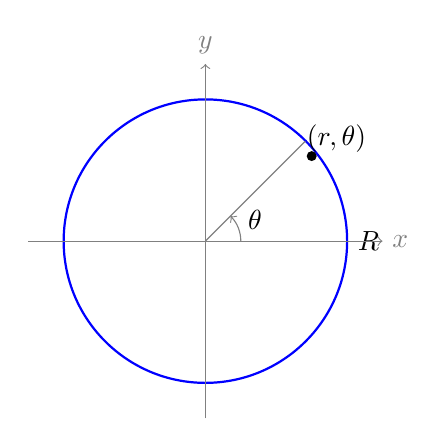
\begin{tikzpicture}[scale=0.9]
    % 圆
    \draw[blue, thick] (0, 0) circle (2);
    
    % 半径
    \draw[gray] (0, 0) -- (2, 0);
    \draw[gray] (0, 0) -- (1.41, 1.41);
    
    % 点
    \fill (1.5, 1.2) circle (2pt);
    
    % 标注
    \draw[->, gray] (0.5, 0) arc (0:45:0.5);
    \node at (0.7, 0.3) {$\theta$};
    
    \node at (1.85, 1.45) {$(r, \theta)$};
    \node at (2.3, 0) {$R$};
    
    % 坐标轴
    \draw[->, gray] (-2.5, 0) -- (2.5, 0) node[right] {$x$};
    \draw[->, gray] (0, -2.5) -- (0, 2.5) node[above] {$y$};
\end{tikzpicture}
\caption{圆域问题}
\label{fig:circular-domain}
\end{figure}

拉普拉斯方程在极坐标下：
\begin{equation}
    \frac{\partial^2 u}{\partial r^2} + \frac{1}{r}\frac{\partial u}{\partial r} + \frac{1}{r^2}\frac{\partial^2 u}{\partial \theta^2} = 0
\end{equation}

设 $u(r, \theta) = R(r)\Theta(\theta)$，分离变量：
\begin{align}
    \Theta''(\theta) + \lambda\Theta(\theta) &= 0 \\
    r^2R''(r) + rR'(r) - \lambda R(r) &= 0
\end{align}

由周期性条件 $\Theta(\theta + 2\pi) = \Theta(\theta)$ 得 $\lambda = n^2$，$n = 0, 1, 2, \ldots$

本征函数：
\begin{equation}
    \Theta_n(\theta) = \begin{cases}
        1, & n = 0 \\
        A_n\cos n\theta + B_n\sin n\theta, & n \geq 1
    \end{cases}
\end{equation}

$R$ 方程是欧拉方程，解为：
\begin{equation}
    R_n(r) = \begin{cases}
        C_0 + D_0\ln r, & n = 0 \\
        C_n r^n + D_n r^{-n}, & n \geq 1
    \end{cases}
\end{equation}

对于圆内问题，要求 $r = 0$ 处有限，故 $D_n = 0$。

解为：
\begin{equation}
    u(r, \theta) = \frac{a_0}{2} + \sum_{n=1}^{\infty}\left(\frac{r}{R}\right)^n\left(a_n\cos n\theta + b_n\sin n\theta\right)
\end{equation}

其中系数由边界条件 $u(R, \theta) = f(\theta)$ 确定：
\begin{equation}
    a_n = \frac{1}{\pi}\int_0^{2\pi} f(\theta)\cos n\theta\,\mathrm{d}\theta, \quad b_n = \frac{1}{\pi}\int_0^{2\pi} f(\theta)\sin n\theta\,\mathrm{d}\theta
\end{equation}

\begin{jinshi}
圆内问题和圆外问题不能混为一谈。只要研究区域包含 $r = 0$，就必须剔除 $\ln r$ 与 $r^{-n}$ 这类在原点发散的项；如果研究的是圆外区域，保留下来的往往恰恰是另一类项。
\end{jinshi}

\begin{lizi}{}{}
求半径为 $R$ 的圆形区域内的静电势。设圆周上的电势为
\begin{equation}
    u(R, \theta) = V_0\cos\theta
\end{equation}
求区域内的电势分布。

\begin{jie}
边界函数只含有 $n = 1$ 的余弦项，因此
\begin{equation}
    a_1 = V_0, \quad a_n = 0 \quad (n \neq 1), \quad b_n = 0
\end{equation}

代入圆内问题的一般解，得
\begin{equation}
    u(r, \theta) = V_0\frac{r}{R}\cos\theta
\end{equation}

这个解在 $r = 0$ 处有限，满足圆内问题对原点的要求。

若改写成直角坐标，由 $x = r\cos\theta$ 得
\begin{equation}
    u(x, y) = \frac{V_0}{R}x
\end{equation}

这表明圆内电势是线性的，对应一个近似均匀的电场。它也和第二章中的复变函数观点完全一致，因为这里的势函数正是解析函数
\begin{equation}
    f(z) = \frac{V_0}{R}z
\end{equation}
的实部。
\end{jie}
\end{lizi}

% ========== 第六节 ==========
\section{非齐次方程的处理}

\subsection{固有函数展开法}

对于非齐次方程
\begin{equation}
    \frac{\partial u}{\partial t} = a^2\frac{\partial^2 u}{\partial x^2} + f(x, t)
\end{equation}

设解的形式为
\begin{equation}
    u(x, t) = \sum_{n=1}^{\infty} T_n(t)\sin\frac{n\pi x}{l}
\end{equation}

将非齐次项也展开：
\begin{equation}
    f(x, t) = \sum_{n=1}^{\infty} f_n(t)\sin\frac{n\pi x}{l}
\end{equation}

代入方程得到 $T_n(t)$ 的常微分方程：
\begin{equation}
    T_n'(t) + \left(\frac{n\pi a}{l}\right)^2 T_n(t) = f_n(t)
\end{equation}

用积分因子法求解。

\begin{lizi}{}{}
求解非齐次热传导方程：
\begin{equation}
    \begin{cases}
        u_t = u_{xx} + \sin x, \quad 0 < x < \pi, \; t > 0 \\
        u(0, t) = u(\pi, t) = 0 \\
        u(x, 0) = 0
    \end{cases}
\end{equation}

\begin{jie}
    用固有函数展开法。设
    \begin{equation}
        u(x, t) = \sum_{n=1}^{\infty} T_n(t)\sin(nx)
    \end{equation}

    将非齐次项 $\sin x$ 展开：只有 $n = 1$ 项，$f_1(t) = 1$。

    代入方程，$T_n(t)$ 满足：
    \begin{equation}
        T_n'(t) + n^2 T_n(t) = \begin{cases} 1, & n = 1 \\ 0, & n \geq 2 \end{cases}
    \end{equation}

    对于 $n = 1$：$T_1' + T_1 = 1$，解得 $T_1(t) = 1 - \mathrm{e}^{-t}$（由初值 $T_1(0) = 0$）。

    对于 $n \geq 2$：$T_n' + n^2 T_n = 0$，由 $T_n(0) = 0$ 得 $T_n(t) = 0$。

    解为
    \begin{equation}
        u(x, t) = (1 - \mathrm{e}^{-t})\sin x
    \end{equation}

    \textbf{稳态}：当 $t \to \infty$ 时，$u \to \sin x$，这是方程 $u_{xx} + \sin x = 0$ 在齐次边界条件下的稳态解。
\end{jie}
\end{lizi}

% ========== 本章小结 ==========
\section{本章小结}

\subsection{分离变量法\index{分离变量法}的步骤}

\begin{enumerate}
    \item 设 $u = X(x)Y(y)T(t)\cdots$
    \item 代入方程，分离变量
    \item 解本征值问题
    \item 解时间/空间方程
    \item 叠加所有特解
    \item 用初始/边界条件确定系数
\end{enumerate}

\subsection{本征值问题的结果}

\begin{table}[htbp]
\centering
\begin{tabular}{llll}
\toprule
\textbf{边界条件} & \textbf{本征值} & \textbf{本征函数} \\
\midrule
$X(0) = X(l) = 0$ & $\left(\frac{n\pi}{l}\right)^2$ & $\sin\frac{n\pi x}{l}$，$n = 1, 2, \ldots$ \\
$X'(0) = X'(l) = 0$ & $\left(\frac{n\pi}{l}\right)^2$ & $\cos\frac{n\pi x}{l}$，$n = 0, 1, 2, \ldots$ \\
$X(0) = X'(l) = 0$ & $\left[\frac{(2n+1)\pi}{2l}\right]^2$ & $\sin\frac{(2n+1)\pi x}{2l}$，$n = 0, 1, \ldots$ \\
\bottomrule
\end{tabular}
\end{table}

% ========== 习题 ==========
\section{习题}

\textbf{基础题}

\begin{enumerate}
    \item 求解：
    \begin{equation}
        \begin{cases}
            u_{tt} = a^2 u_{xx}, \quad 0 < x < \pi \\
            u(0, t) = u(\pi, t) = 0 \\
            u(x, 0) = \sin 2x, \quad u_t(x, 0) = 0
        \end{cases}
    \end{equation}
    
    \item 求解热传导方程：
    \begin{equation}
        \begin{cases}
            u_t = u_{xx}, \quad 0 < x < 1, \; t > 0 \\
            u(0, t) = u(1, t) = 0 \\
            u(x, 0) = x(1-x)
        \end{cases}
    \end{equation}
\end{enumerate}

\textbf{综合题}

\begin{enumerate}[resume]
    \item 求解有界弦振动，边界条件为 $u_x(0, t) = u_x(l, t) = 0$（自由端）：
    \begin{equation}
        \begin{cases}
            u_{tt} = a^2 u_{xx}, \quad 0 < x < l \\
            u_x(0, t) = u_x(l, t) = 0 \\
            u(x, 0) = \cos\frac{\pi x}{l}, \quad u_t(x, 0) = 0
        \end{cases}
    \end{equation}
    
    \item 在矩形区域 $0 < x < a$，$0 < y < b$ 上求解拉普拉斯方程，边界条件为：
    \begin{equation}
        u(0, y) = u(a, y) = 0, \quad u(x, 0) = 0, \quad u(x, b) = \sin\frac{\pi x}{a}
    \end{equation}
    
    \item 在圆域 $r < R$ 内求解拉普拉斯方程，边界条件为 $u(R, \theta) = \cos\theta$。
\end{enumerate}

\textbf{挑战题}

\begin{enumerate}[resume]
    \item 证明：本征函数系的正交性。
    
    \item 求解非齐次问题：
    \begin{equation}
        \begin{cases}
            u_t = u_{xx} + \sin\pi x, \quad 0 < x < 1 \\
            u(0, t) = u(1, t) = 0 \\
            u(x, 0) = 0
        \end{cases}
    \end{equation}
\end{enumerate}
